This chapter applies the theoretical framework of Mandelstam and Tamm's Quantum Speed Limit discussed in the methodology to a specific two-state quantum system.

\section{System Hamiltonian and Time Evolution}
Consider a two-state quantum system governed by the Hamiltonian:
\begin{equation}
    H = \frac{\hbar \omega_0}{2} \sigma_z = \frac{\hbar \omega_0}{2} \begin{pmatrix} 1 & 0 \\ 0 & -1 \end{pmatrix}
\end{equation}
where $\sigma_z$ is the Pauli Z matrix. This time-independent, diagonal Hamiltonian is the standard model for a two-level system, such as a spin-1/2 particle in a constant magnetic field. Its simplicity provides exact analytical solutions for state evolution and energy variance, making it ideal for clearly demonstrating the Mandelstam-Tamm bound.

To compute how the system changes over time, we use the unitary time evolution operator $U(t)$. In quantum mechanics, a unitary operator (where $U^\dagger U = I$) is fundamental because it strictly preserves the inner product and the norm of state vectors, ensuring that total probability is perfectly conserved. By applying $U(t)$, we can deterministically rotate the initial state through the Hilbert space. This unitary preservation is what mathematically allows us to accurately track the survival probability and Bures angle. For this time-independent Hamiltonian, the evolution operator is given by:
\begin{equation}
    U(t) = e^{-i H t / \hbar} = \begin{pmatrix} e^{-i \omega_0 t / 2} & 0 \\ 0 & e^{i \omega_0 t / 2} \end{pmatrix}
\end{equation}

\section{Energy Variance and the MT Bound}
To apply the Mandelstam-Tamm bound, we first compute the energy variance $\Delta H$ of the initial state. The expectation value of the Hamiltonian is:
\begin{equation}
    \langle H \rangle = \langle \psi(0) | H | \psi(0) \rangle = \frac{\hbar \omega_0}{2} \left( \cos^2\frac{\theta}{2} - \sin^2\frac{\theta}{2} \right) = \frac{\hbar \omega_0}{2} \cos\theta
\end{equation}
Since $H^2 = \left(\frac{\hbar \omega_0}{2}\right)^2 I$, the expectation value of $H^2$ is simply $\langle H^2 \rangle = \left(\frac{\hbar \omega_0}{2}\right)^2$. 
Taking the square root of the energy variance yields the standard deviation $\Delta H$, representing the state's energy uncertainty:
\begin{equation}
    \Delta H = \sqrt{\langle H^2 \rangle - \langle H \rangle^2} = \sqrt{\left(\frac{\hbar \omega_0}{2}\right)^2 - \left(\frac{\hbar \omega_0}{2} \cos\theta\right)^2} = \frac{\hbar \omega_0}{2} \sin\theta
\end{equation}

According to the Mandelstam-Tamm bound, the time $\Delta t$ required for the system to evolve to a state separated by a Bures angle $\Theta$ from the initial state is bounded by:
\begin{equation}
    t \ge \frac{\hbar \Theta}{\Delta H} = \frac{\hbar \Theta}{\frac{\hbar \omega_0}{2} \sin\theta} = \frac{2 \Theta}{\omega_0 \sin\theta}
\end{equation}
For the system to reach an orthogonal state, the distance is $\Theta = \pi/2$. The minimum time required to reach this orthogonal state is thus:
\begin{equation}
    t \ge \frac{2 \cdot (\pi/2)}{\omega_0 \sin\theta} \implies \tau_{QSL} = \frac{\pi}{\omega_0 \sin\theta}
\end{equation}
This indicates that the speed of evolution depends on the initial state parameter $\theta$. The fastest evolution to an orthogonal state occurs when $\theta = \pi/2$ (states on the equator of the Bloch sphere), yielding a minimum time of $\tau_{QSL} = \pi/\omega_0$.

The Bloch sphere is a geometrical representation of the pure state space of a two-level quantum mechanical system (a qubit). The north and south poles represent the mutually orthogonal computational basis states $|0\rangle$ and $|1\rangle$, while any point on the equator ($\theta = \pi/2$) represents an equal superposition of these basis states \cite{jazaeri2019}. 
\begin{figure}[ht]
    \centering
    \includegraphics[width=0.45\textwidth]{"figures/Bloch Sphere"}
    \caption{The Bloch sphere representation of a two-level quantum system state. Figure adapted from \cite{jazaeri2019}.}
    \label{fig:bloch_sphere}
\end{figure}

\section{Generalized Mandelstam-Tamm Bound}
Let the initial state of the system be parameterized by an angle $\theta$ on the Bloch sphere:
\begin{equation}
    |\psi(0)\rangle = \cos\frac{\theta}{2} |0\rangle + \sin\frac{\theta}{2} |1\rangle
\end{equation}
The state at a later time $t$ is:
\begin{equation}
    |\psi(t)\rangle = U(t) |\psi(0)\rangle = \cos\frac{\theta}{2} e^{-i \omega_0 t / 2} |0\rangle + \sin\frac{\theta}{2} e^{i \omega_0 t / 2} |1\rangle
\end{equation}

The inner product between the initial and evolved state is:
\begin{equation}
    \langle \psi(0) | \psi(t) \rangle = \cos^2\frac{\theta}{2} e^{-i \omega_0 t / 2} + \sin^2\frac{\theta}{2} e^{i \omega_0 t / 2} = \cos\left(\frac{\omega_0 t}{2}\right) - i \cos\theta \sin\left(\frac{\omega_0 t}{2}\right)
\end{equation}
The squared magnitude of this overlap gives the fidelity:
\begin{equation}
    |\langle \psi(0) | \psi(t) \rangle|^2 = \cos^2\left(\frac{\omega_0 t}{2}\right) + \cos^2\theta \sin^2\left(\frac{\omega_0 t}{2}\right)
\end{equation}

The Bures angle $\alpha(t)$ between the initial and evolved state is defined as:
\begin{equation}
    \alpha(t, \theta) = \arccos\left(|\langle \psi(0) | \psi(t) \rangle|\right) = \arccos\sqrt{\cos^2\left(\frac{\omega_0 t}{2}\right) + \cos^2\theta \sin^2\left(\frac{\omega_0 t}{2}\right)}
\end{equation}

Furthermore, adding an arbitrary relative phase $\phi$ to the initial state:
\begin{equation}
    |\psi(0)\rangle = \cos\frac{\theta}{2} |0\rangle + e^{i\phi}\sin\frac{\theta}{2} |1\rangle
\end{equation}
shows that $e^{i\phi}$ cancels during the inner product calculation. So, $\alpha(t)$ is independent of $\phi$.

\subsection{Equatorial Pure States and Bound Saturation}
To determine which initial pure states can ever evolve into a completely orthogonal state ($\alpha = \pi/2$), we must set the argument of the arccosine to zero:
\begin{equation}
    \cos^2\left(\frac{\omega_0 t}{2}\right) + \cos^2\theta \sin^2\left(\frac{\omega_0 t}{2}\right) = 0
\end{equation}
Because this is a sum of two non-negative squares, both terms must equal zero simultaneously. The first term dictates that $\cos(\omega_0 t / 2) = 0$, meaning the minimum time to reach orthogonality is $t = \pi/\omega_0$. At this specific time, $\sin^2(\omega_0 t / 2) = 1$. Consequently, for the second term to vanish, we must have $\cos\theta = 0$, which strictly restricts the initial state to $\theta = \pi/2$. 

This mathematical condition reveals a profound physical property: only the specific family of pure states lying exactly on the equator of the Bloch sphere can ever reach a state completely orthogonal to themselves. For these equatorial states, the time-dependent Bures angle simplifies perfectly to a linear function:
\begin{equation}
    \alpha\left(t, \theta = \frac{\pi}{2}\right) = \frac{\omega_0 t}{2}
\end{equation}

Crucially, we can show that the Mandelstam-Tamm bound saturates (reaches equality) for this specific family of states. Substituting $\theta = \pi/2$ into our earlier energy variance equation gives the maximum possible uncertainty $\Delta H = \hbar \omega_0 / 2$. The theoretical Quantum Speed Limit time to reach an orthogonal state ($\Theta = \pi/2$) is therefore:
\begin{equation}
    \tau_{QSL} = \frac{\pi \hbar}{2 \Delta H} = \frac{\pi \hbar}{2 (\hbar \omega_0 / 2)} = \frac{\pi}{\omega_0}
\end{equation}
This strictly matches the dynamical time $t = \pi/\omega_0$ derived above, proving that equatorial pure states evolve at the absolute maximum physical speed permitted by quantum mechanics.

\section{Computational Analysis}
We used Python to plot the Bures angle $\alpha(t)$ against dimensionless time $\omega_0 t$ for various initial states ($\theta$) to analyze the generalized MT bound.

\begin{figure}[ht]
    \centering
    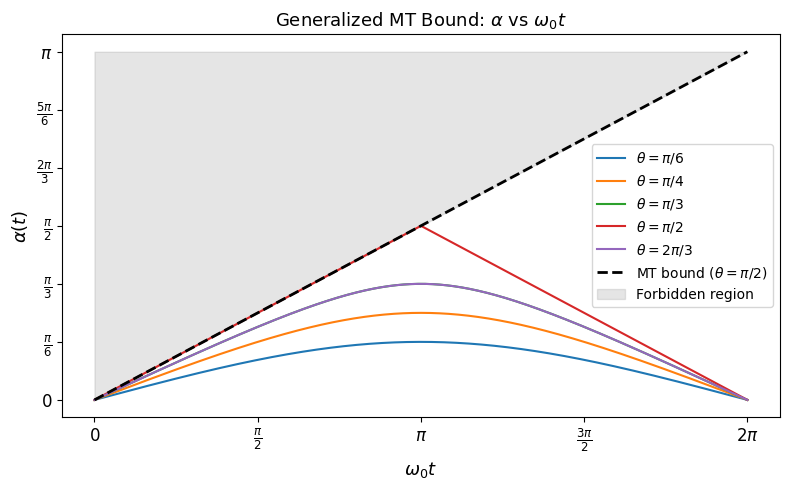
\includegraphics[width=0.8\textwidth]{figures/Generalized_MT_Bound.png}
    \caption{Generalized Mandelstam-Tamm Bound: $\alpha(t)$ vs $\omega_0 t$ for different initial states $\theta$. The black dashed line represents the MT bound for orthogonal states ($\theta = \pi/2$), and the shaded gray region is forbidden by the bound.}
    \label{fig:mt_bound}
\end{figure}

Figure \ref{fig:mt_bound} provides a comprehensive visualization of the system's evolution for various initial states, defined by different values of the polar angle $\theta$ on the Bloch sphere, ranging from the poles ($\theta=0$) to the equator ($\theta=\pi/2$). The horizontal axis represents dimensionless time $\omega_0 t$. Using dimensionless time allows the plot to be universally applicable, meaning the fundamental shape of the curves remains the same regardless of the specific physical value of the natural frequency $\omega_0$. 

The plot prominently features a straight diagonal dashed line. This diagonal represents the absolute maximum rate of evolution permitted by the Mandelstam-Tamm bound. Because the generalized bound states $\alpha \le \Delta H t / \hbar$, and the maximum energy variance is $\Delta H = \hbar \omega_0 / 2$, this limiting diagonal has a mathematical slope of exactly $1/2$ (where $\alpha = \omega_0 t / 2$). The shaded gray area above this diagonal is the forbidden region. No physical quantum state can evolve fast enough to cross into this area, as doing so would violate the fundamental energy-time uncertainty principle.

Every curve exhibits a smooth, periodic oscillation. This sinusoidal shape directly reflects the unitary nature of the time evolution operator. Physically, the state vector is continuously precessing around the z-axis of the Bloch sphere. Due to this continuous uniform rotation, the state periodically reaches a point of maximum distinguishability at half the oscillation period (when $\omega_0 t = \pi$) before smoothly rotating back to its exact initial configuration to complete the cycle.

Furthermore, the curves clearly show that only the equatorial states ($\theta = \pi/2$) evolve fast enough to touch the diagonal bound and successfully reach a completely orthogonal state ($\alpha = \pi/2$). As the initial state parameter $\theta$ decreases toward $0$, the curves become progressively flatter. This flattening occurs because moving closer to the poles of the Bloch sphere decreases the energy variance $\Delta H$. With less energy uncertainty, the system is strictly forced to evolve more slowly, which fundamentally limits the maximum Bures angle it can ever reach. In the extreme case where $\theta = 0$, the state is an energy eigenstate (a stationary state) with zero variance, and the curve remains perfectly flat at $\alpha = 0$ to indicate that no state evolution occurs.
